\subsection{Stochastic Uncertainty Injecting Scheme}
For each sampled edge $e$ with the distributed standard deviation $\sigma_{e}$, we select the probability deviation $r_{e}$ where $r_{e} \leftarrow R_{\sigma_{e}}$. 
Thus, the remaining question is \emph{how can we safely alter edge probability for higher anonymity?}
Given the deterministic graph, the idea of uncertainty injecting is to transfer probabilities from existing edges to potential edges, as outlined in Equation~1.
However, the uncertainty injecting scheme is unexplored in the uncertain scenario.  
\begin{figure}[!htb]
  \centering
        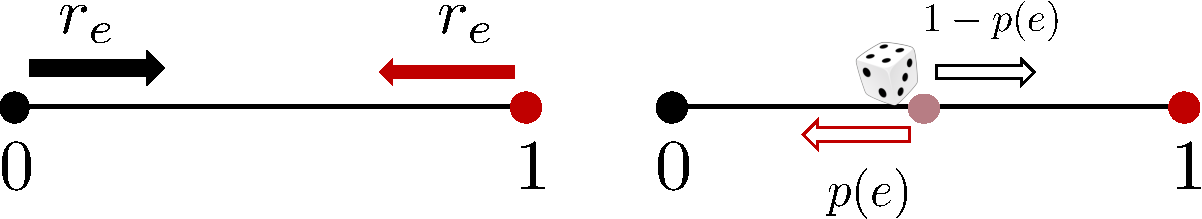
\includegraphics[width=\linewidth]{ill/shift_UI.pdf}
    \caption{The generalized uncertainty injecting scheme.}
\end{figure}
There are many potential ways to extend the uncertain injecting scheme to the probabilistic context.   
One option is the Most-Provable-Scheme where the edge probability alteration follows the most probable policy.
\begin{equation*}
  p(e) =
  \begin{cases}
     p(e)-r_{e}    & p(e) \ge 0.5 \\
     p(e)+r_{e}    & otherwise 
  \end{cases}
  \label{eq:inject}
\end{equation*}

Another simple alternative is to consider the probability the edge exists as an indicator of the scheme. 
It performs the following uncertainty injecting scheme.
\begin{align}
  p(e)~&=~ [p(e)] \cdot (1-r_{e})+ [1-p(e)] \cdot r_{e} \\
      ~&=~ p(e) + \big[ 1- 2 p(e) \big] \cdot r_{e}
  \label{eq:ui}
\end{align}
It has already been used as the uncertainty injecting scheme in our previous work~\cite{Xiao:2018}; 
The flexible value of the edge probability is limited to the range between $p(e)$ and $1-p(e)$.
Intuitively, it requires maximizing degree entropy/variance. 
% The intuitive interpretation is XXXXX. 

However, its connection to the core anonymity objective and the mathematical foundation are unclear. 
In this work, we show the stochastic uncertainty injecting scheme can maximize the related objective function of anonymity.  

\textbf{The relaxed version of anonymity}~~
To simplify the discussion, let us consider the primary case $k$-obf which low bounds the entropy of posterior-probability distribution over all the nodes.  
It imposes a set of hard constraints on the output solution. 
To make it formal, let us define the set of feasible solutions satisfying all the constraints as:
\begin{equation*}
  \{\pg~~s.t.~~ \forall v ~\mathrm{E}(v) \ge  \log k \}. 
\end{equation*}
$k-$obf can be expressed as joint satisfaction of a set of constraints 
since the uncertain graph is said to be $k$-obf iff it $k-$obfuscates all the nodes. 
Then, in order to sanitize graph, we could maximize the following function: 
\begin{equation*}
    \mathcal{F}_{e} = \prod_{v \in V} \mathcal{C}_{v}              
\end{equation*} 
where 
\begin{equation*}
  \mathcal{C}_{v} = 
  \begin{cases}
    1 & \mathrm{E}_{v} \ge  \log k \\ 
    0 & otherwise 
  \end{cases}
\end{equation*}

The single constraint {\Constraint} is either fully satisfied or thoroughly violated. 
The discontinuity limits the opportunity of gradient-based optimization methods.
The connection between our objective function is still unclear.  
Thus, we relax the single constraint {\Constraint} to a fuzzy relation as: 
\begin{equation*}
  \mathcal{C}_{v} = e^{\mathcal{E}_{v}-\lambda}.
\end{equation*}
Then, the satisfaction becomes a continuous and differential function {\wrt} the entropy. 
It turns out that the problem can be reduced to maximizing a much simpler function with the relaxed version of anonymity.  

\begin{observation}
  The maximization of $\mathcal{F}_{e}$ is equivalent to the maximization of the following function:
  \begin{equation*}
    \mathcal{F} =  \sum_{v\in V} E(v) - \Number E(\Omega)
  \end{equation*}
\end{observation}
Targeting at high utility, it aims at increasing the uncertainty at the vertex level $\sum_{v \in V} E(v)$. 

\textbf{Proof Sketch.}~~
Let $\Omega$ presents the domain of property values in the given graph; we can see that 
\begin{equation*}
  \mathcal{F}_{e} = \prod_{\omega \in \Omega} \underbrace{\mathcal{C}_{\omega} \ldots \mathcal{C}_{\omega}}_{s(\omega)}, 
\end{equation*}
Taking logarithm for both sides and combining the approximation, our goal is actually to maximized 
\begin{align*}
  \log \mathcal{F}_{e} &= \sum_{\omega \in \Omega} s(\omega)~\log C(\omega) \\
                       &= \sum_{\omega \in \Omega} s(\omega) \big[ E(\omega) - \lambda \big] \\
                       &= \sum_{\omega \in \Omega} s(\omega) E(\omega) ~-~ \Number \lambda 
\end{align*}
Therefore, after removing the constant $\Number\lambda$, our goal is actually to maximize 
$\sum_{\omega \in \Omega} s(\omega) E(\omega)$. 
It bridges the anonymity of the overall graph $\mathcal{F}_{e}$ 
with the component coding (the disorder) of the fuzzy matching matrix. 

To perform data coding, we have two angles, row  and column, that gain the same result of coding length $\mathcal{L}$ as:
\begin{align*}
  \mathcal{L} &= \sum_{v \in V} E(v) + \Number \log \Number                             &(row)\\
              &= \sum_{\omega \in \Omega} s(\omega) E(\omega)~+~\Number E(\Omega) &(column). 
\end{align*}
Therefore, after removing the constant $\Number \log \Number$, our goal is actually to maximize 
$\mathcal{F}_{e}$. $\square$  

\begin{observation}
  Equation~\ref{eq:ui} approximates the gradient-based exploration of the simplified objective function $F$.
\end{observation}

\textbf{Proof Sketch.}~~
Fix such node $v \in \mathcal{G}$ and let $e_{1},\ldots, e_{l}$ be $l$ edges that include $v$. 
Letting $d_{v}$ be the random variable corresponding to the degree of $v$, 
we have 
\begin{equation*}
  d_{v} ~=~ \sum_{i}^{l} p(e_{i}). 
\end{equation*}
As ever described, {\methodName} selectively modifies edges connected to unique nodes ({\ie}, nodes with high degree).
The degree of such node $v$ can be approximated by the normal distribution. (The Central Limit Theorem becomes effective already for $l\approx 30$; for unique nodes in the real uncertain graph, the approximation becomes accurate enough.) We have
\vspace{-5pt}
\begin{align*}
   d_{v}~&\sim~\mathcal{N}(u, \sigma^2); \\
   \sigma^{2}~&=~\sum_{i=1}^{l} Var(P(e_{i}))=\sum_{i=1}^{l} p(e_{i}) (1-p(e_{i}))
   \vspace{-15pt}
\end{align*}
The entropy of the random variable, $E(v)$, can then be approximated by the differential entropy of the normal distribution as ${{1}\over{2}}{\ln (2\pi\sigma^2)}+ {{1}\over{2}}$. 
The gradient of our objective function {\wrt} the edge existence  can be rewritten as
\begin{align*} 
  \nabla \mathcal{F}~&=~\nabla E_{v}~=~\nabla \ln(\sigma^2) \\
                    ~&\sim \frac{1}{\sigma^2} \nabla \sigma^{2}~\sim~\frac{1}{\sigma^2} \big [ 1-2~p(e_{i}) \big].~\square
\end{align*}